\documentclass[11pt,letterpaper]{article}
\usepackage[utf8]{inputenc}

%----- Configuración del estilo del documento------%
\usepackage[table]{xcolor}
\usepackage{epsfig,graphicx}
\usepackage[left=2cm,right=2cm,top=1.8cm,bottom=2.3cm]{geometry}
\usepackage{fancyhdr}
\usepackage{lastpage}
\pagestyle{fancy}
\fancyhf{}
\rfoot{\textit{Página \thepage \hspace{1pt} de \pageref{LastPage}}}
\usepackage{array}

%------ Paquetes matemáticos básicos --------%
\usepackage{amsmath}
\usepackage{amssymb}
\usepackage{amsthm}

%------ Texto aleatorio ----- %

\usepackage{lipsum}



\begin{document}

%------ Encabezado -------- %

\begin{center}
    \begin{minipage}{3cm}
    	\begin{center}
    		\includegraphics[height=3.4cm]{./imagenes/logo_unam.png}
    	\end{center}
    \end{minipage}\hfill
    \begin{minipage}{10cm}
    	\begin{center}
    	\textbf{\large Universidad Nacional Autónoma de México}\\[0.1cm]
        \textbf{Facultad de Ciencias}\\[0.1cm]
        \textbf{Estructuras Discretas $|$ Grupo 7020}\\[0.1cm]
        \textbf{Tarea 2: Lógica Preposicional}\\[0.1cm]
        Real Araiza Yamile\\[0.1cm]
        Tenorio Reyes Ihebel Luro\\[0.1cm]
        12/Oct/2024
    	\end{center}
    \end{minipage}\hfill
    \begin{minipage}{3cm}
    	\begin{center}
    		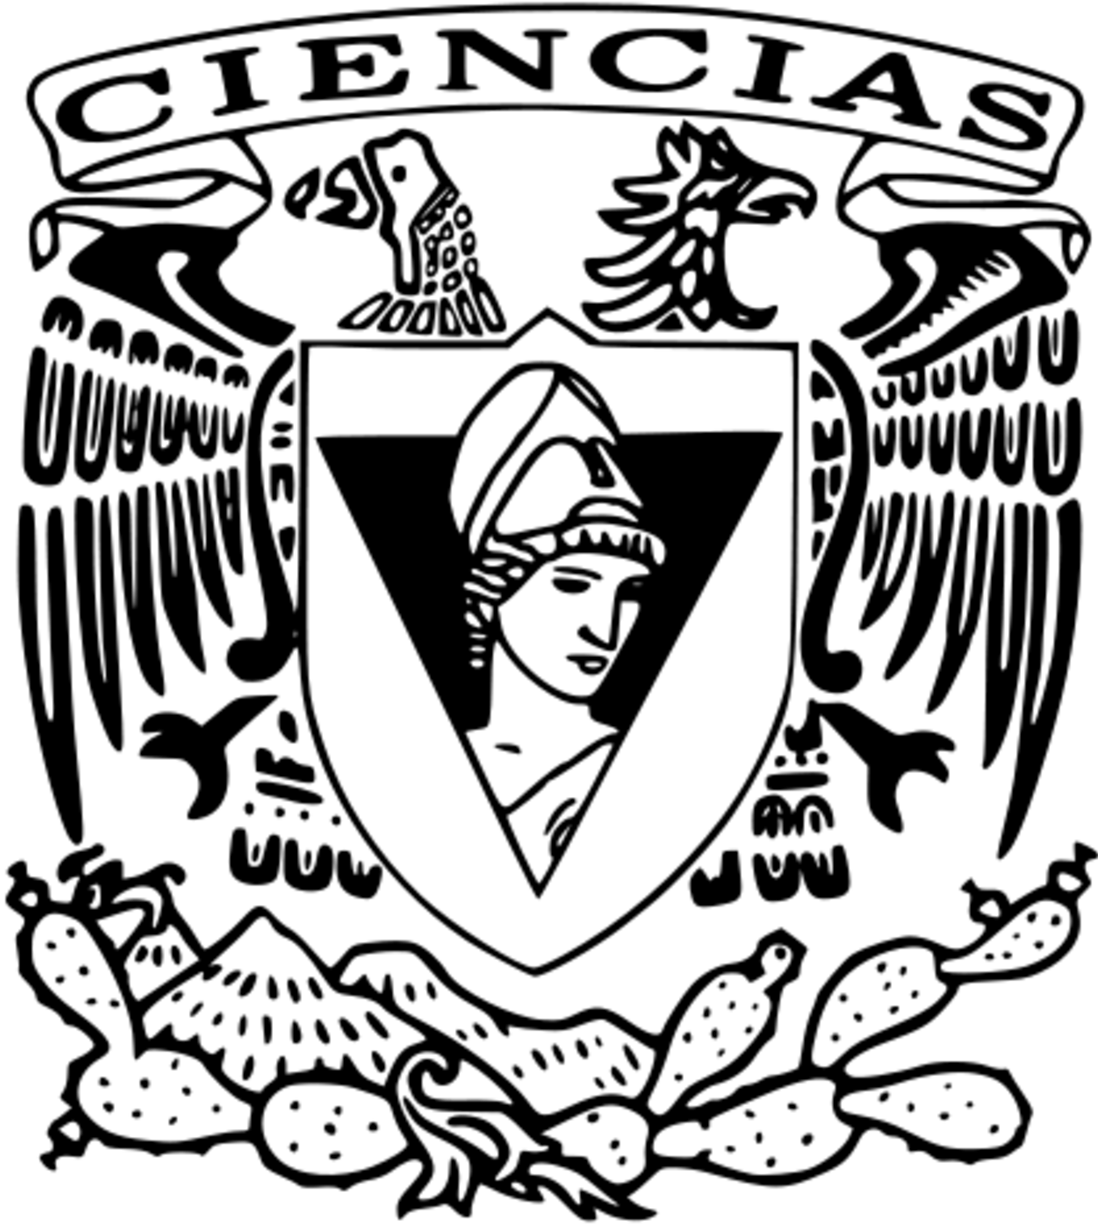
\includegraphics[height=3.4cm]{./imagenes/Logo_FC.png}
    	\end{center}
    \end{minipage}
\end{center}

\rule{17cm}{0.1mm}

%------ Fin de encabezado -------- %



%====== Ejercicio 01 ======%
\section*{1. Asumiendo los axiomas de un algebra booleana A = \{\{0,1\},+,·\} demostrar las siguientes propiedades:}
\section*{Demostraciones}

\subsection*{a) Idempotencia}

Para la idempotencia de la suma: \( x + x = x \) y \( x \cdot x = x \).

\textbf{Para \( x + x = x \):}

\[\begin{aligned}
x + x &= x + x \cdot 1 & \text{(ya que 1 es el elemento neutro del producto)} \\
      &= x + x \cdot \overline{x} & \text{(por el complemento: \( x \cdot \overline{x} = 0 \))} \\
      &= x \cdot (1 + \overline{x}) & \text{(por distributividad)} \\
      &= x \cdot 1 = x.
\end{aligned}
\]

\textbf{Para \( x \cdot x = x \):}

\[
\begin{aligned}
x \cdot x &= x \cdot x + 0 & \text{(agregando el neutro aditivo)} \\
          &= x \cdot x + x \cdot \overline{x} & \text{(ya que \( x \cdot \overline{x} = 0 \))} \\
          &= x \cdot (x + \overline{x}) & \text{(por factorización usando la distributividad)} \\
          &= x \cdot 1 & \text{(dado que \( x + \overline{x} = 1 \))} \\
          &= x.
\end{aligned}
\]

\subsection*{b) Idempotencia del complemento}

Para demostrar que \( \overline{\overline{x}} = x \), usamos que el complemento satisface \( x + \overline{x} = 1 \) y \( x \cdot \overline{x} = 0 \).

\[
\begin{aligned}
\overline{\overline{x}} &= x + 0 & \text{(ya que 0 es el neutro de la suma)} \\
                        &= x + (x \cdot \overline{x}) & \text{(por el complemento: \( x \cdot \overline{x} = 0 \))} \\
                        &= x \cdot 1 = x.
\end{aligned}
\]

\subsection*{c) Elemento dominante}

Para \( x + 1 = 1 \) y \( x \cdot 0 = 0 \):

\textbf{Para \( x + 1 = 1 \):}

\[
\begin{aligned}
x + 1 &= (x + 1) \cdot 1 & \text{(por el elemento neutro del producto)} \\
      &= (x + 1) \cdot (x + \overline{x}) & \text{(por complemento: \( x + \overline{x} = 1 \))} \\
      &= x + 1 = 1.
\end{aligned}
\]

\textbf{Para \( x \cdot 0 = 0 \):}

\[
\begin{aligned}
x \cdot 0 &= x \cdot (x \cdot \overline{x}) & \text{(ya que \( x \cdot \overline{x} = 0 \))} \\
          &= (x \cdot x) \cdot \overline{x} & \text{(por asociatividad)} \\
          &= x \cdot \overline{x} & \text{(ya que \( x \cdot x = x \) por idempotencia)} \\
          &= 0.
\end{aligned}
\]

Esto es directo por la propiedad de absorción del producto con el elemento neutro \( 0 \).

\subsection*{d) Absorción}

Para \( x + x \cdot y = x \) y \( x \cdot (x + y) = x \):

\textbf{Para \( x + x \cdot y = x \):}

\[
\begin{aligned}
x + x \cdot y &= x \cdot 1 + x \cdot y & \text{(por el elemento neutro de la suma)} \\
              &= x \cdot (1 + y) & \text{(por distributividad)} \\
              &= x.
\end{aligned}
\]

\textbf{Para \( x \cdot (x + y) = x \):}

\[
\begin{aligned}
x \cdot (x + y) &= x \cdot x + x \cdot y & \text{(por distributividad)} \\
                &= x + x \cdot y = x. & \text{(por la propiedad de absorción)}
\end{aligned}
\]



%====== Ejercicio 02 ======%
\section*{Dibuja los circuitos lógicos para las siguientes expresiones:}
\subsection*{a) $xyz \oplus x\overline{y}z$}
\begin{center}
  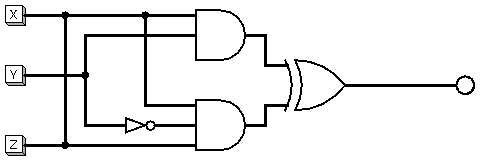
\includegraphics[width=8cm]{./imagenes/Ej2a.png}
\end{center}

\subsection*{b) $xy+x \overline{y} $}
\begin{center}
  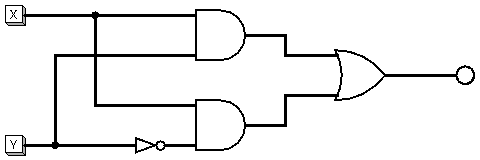
\includegraphics[width=8cm]{./imagenes/Ej2b.png}
\end{center}

\subsection*{c) $xy\overline{z} + x \overline{yz}$}
\begin{center}
  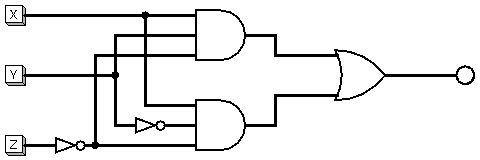
\includegraphics[width=8cm]{./imagenes/Ej2c.png}
\end{center}

\subsection*{d) $\overline{x} + \overline{y} + xyz$}
\begin{center}
  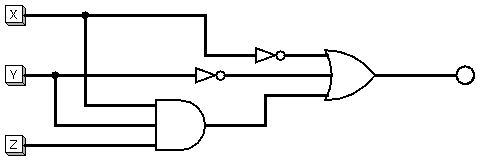
\includegraphics[width=8cm]{./imagenes/Ej2d.png}
\end{center}

%====== Ejercicio 03 ======%
\section*{3. Utilizando mapas de Karnaugh, reducir las siguientes expresiones y dibujar los circuitos reducidos:}

\subsection*{a) Expresión: \( xy + x\overline{y} \)}

\textbf{Mapa de Karnaugh:}\[
\begin{array}{c|cc}
x \setminus y & 0 & 1 \\
\hline
0 & 0 & 0 \\
1 & 1 & 1 \\
\end{array}
\]

Se observa que se pueden agrupar los unos en una fila, lo que reduce la expresión a:
\[
x
\]

\textbf{Expresión reducida:} \( x \)

\textbf{Circuito lógico:} Un solo cable que representa la variable \( x \).

\subsection*{b) Expresión: \( \overline{x}y + \overline{x}\overline{y} \)}

\textbf{Mapa de Karnaugh:}
\[
\begin{array}{c|cc}
x \setminus y & 0 & 1 \\
\hline
0 & 1 & 1 \\
1 & 0 & 0 \\
\end{array}
\]

Los términos se pueden agrupar en la columna de \( \overline{x} \), resultando en:
\[
\overline{x}
\]

\textbf{Expresión reducida:} \( \overline{x} \)

\textbf{Circuito lógico:} Un inversor para la variable \( x \).

\subsection*{c) Expresión: \( xyz + \overline{x}yz \)}

\textbf{Mapa de Karnaugh:}
\[
\begin{array}{c|cccc}
x \setminus yz & 00 & 01 & 11 & 10 \\
\hline
0 & 0 & 0 & 1 & 0 \\
1 & 0 & 0 & 1 & 0 \\
\end{array}
\]

Agrupamos los términos \( xyz \) y \( \overline{x}yz \), lo que da como resultado:
\[
yz
\]

\textbf{Expresión reducida:} \( yz \)

\textbf{Circuito lógico:} Un AND entre \( y \) y \( z \).

\subsection*{d) Expresión: \( xy\overline{z} \ + x\overline{y} \overline{z} \ + \overline{x}y\overline{z} \ + \overline{x}\overline{y} \overline{z} \)}

\textbf{Mapa de Karnaugh:}
\[
\begin{array}{c|cccc}
x \setminus yz & 00 & 01 & 11 & 10 \\
\hline
0 & 1 & 0 & 0 & 1 \\
1 & 1 & 0 & 0 & 1 \\
\end{array}
\]

Se agrupan los unos en la fila de \( \overline{z} \), obteniendo:
\[
\overline{z} \
\]

\textbf{Expresión reducida:} \( \overline{z} \)

\textbf{Circuito lógico:} Un inversor para la variable \( z \).

\subsection*{e) Expresión: \( \overline{x}\overline{y} + \overline{x}y + xy \)}

\textbf{Mapa de Karnaugh:}
\[
\begin{array}{c|cc}
x \setminus y & 0 & 1 \\
\hline
0 & 1 & 1 \\
1 & 0 & 1 \\
\end{array}
\]

Agrupamos los términos en la columna de \( y \), resultando en:
\[
y
\]

\textbf{Expresión reducida:} \( y \)

\textbf{Circuito lógico:} Un solo cable que representa la variable \( y \).

\subsection*{f) Expresión: \( \overline{x}\overline{y} + \overline{x}y + x + y \)}

\textbf{Mapa de Karnaugh:}
\[
\begin{array}{c|cc}
x \setminus y & 0 & 1 \\
\hline
0 & 1 & 1 \\
1 & 1 & 1 \\
\end{array}
\]

Todos los valores son 1, lo que significa que:
\[
1
\]

\textbf{Expresión reducida:} \( 1 \)

\textbf{Circuito lógico:} Una constante lógica de 1.

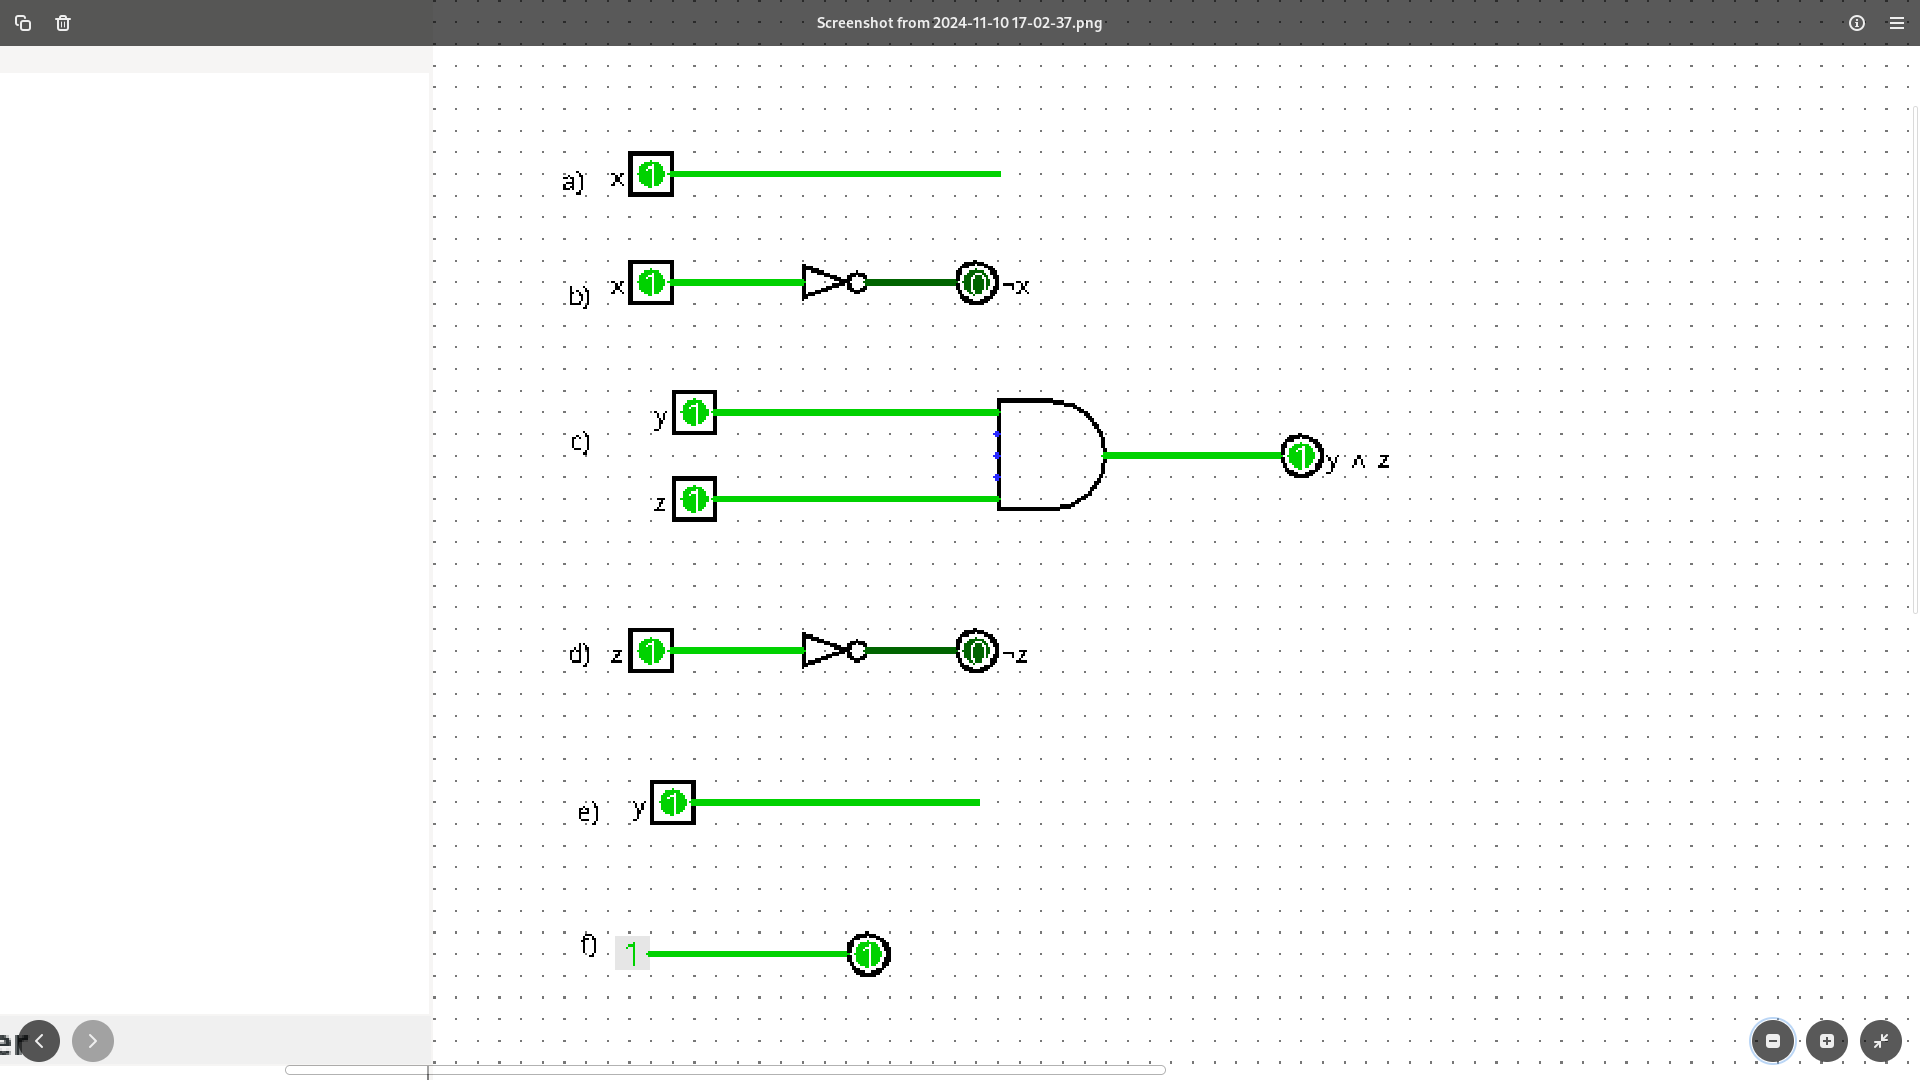
\includegraphics[height=10.0cm]{./imagenes/circuitos.png}




%====== Ejercicio 04 ======%
\section*{Diseñar un circuito decodificador con 4 etradas para la siguiente tabla de verdad, donde - denota cualquier valor, 0 o 1}
\begin{table}[h!]
\centering
\begin{tabular}{| c | c | c | c | | c | c | c |}
\hline
\multicolumn{4}{|c||}{Entradas} & \multicolumn{3}{c|}{Salidas} \\
\hline
0 & 0 & 0 & 0 & - & - & 0 \\
0 & 0 & 0 & 1 & 0 & 0 & 1 \\
0 & 0 & 1 & - & 0 & 1 & 1 \\
0 & 1 & - & - & 1 & 0 & 1 \\
1 & - & - & - & 1 & 1 & 1 \\
\hline
$E_4$ & $E_3$ & $E_2$ & $E_1$ & $S_3$ & $S_2$ & $S_1$ \\
\hline
\end{tabular}
%\caption{Tabla de Entradas y Salidas}
%\label{tab:entradas_salidas}
\end{table}

\begin{center}
  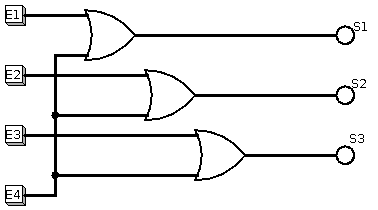
\includegraphics[width=8cm]{./imagenes/Ej4.png}
\end{center}


%====== Ejercicio 05 ======%




%====== Ejercicio 06 ======%
\section*{6. Expresar las siguientes oraciones como formulas de la lógica de predicados; indicar las constantes, las variables, los cuantificadores y su alcance:}

\subsection*{a) "Hay algunos médicos que son odontólogos."}

\textbf{Constantes:} Ninguna \\
\textbf{Variables:} \( x \) (representa personas) \\
\textbf{Cuantificadores:} Existencial (\( \exists \))

\textbf{Fórmula:}
\[
\exists x \, (M(x) \land O(x))
\]

\textbf{Interpretación:} Existe al menos un \( x \) tal que \( x \) es médico \( (M(x)) \) y \( x \) es odontólogo \( (O(x)) \).

\subsection*{b) "Ninguna planta es mamífero o pez."}

\textbf{Constantes:} Ninguna \\
\textbf{Variables:} \( x \) (representa seres vivos) \\
\textbf{Cuantificadores:} Universal (\( \forall \))

\textbf{Fórmula:}
\[
\forall x \, (P(x) \rightarrow \neg (M(x) \lor Z(x)))
\]

\textbf{Interpretación:} Para todo \( x \), si \( x \) es planta \( (P(x)) \), entonces \( x \) no es mamífero \( (M(x)) \) ni pez \( (Z(x)) \).

\subsection*{c) "Cualquiera puede tomarle el pelo a la directora."}

\textbf{Constantes:} Directora (\( D \)) \\
\textbf{Variables:} \( x \) (representa personas) \\
\textbf{Cuantificadores:} Universal (\( \forall \))

\textbf{Fórmula:}
\[
\forall x \, T(x, D)
\]

\textbf{Interpretación:} Para todo \( x \), \( x \) puede tomarle el pelo a la directora \( (T(x, D)) \).

\subsection*{d) "Hay un abogado a quien cualquiera le toma el pelo."}

\textbf{Constantes:} Ninguna \\
\textbf{Variables:} \( x, y \) (representan personas) \\
\textbf{Cuantificadores:} Existencial (\( \exists \)) y Universal (\( \forall \))

\textbf{Fórmula:}
\[
\exists x \, (A(x) \land \forall y \, T(y, x))
\]

\textbf{Interpretación:} Existe al menos un \( x \) tal que \( x \) es abogado \( (A(x)) \) y para todo \( y \), \( y \) le toma el pelo a \( x \) \( (T(y, x)) \).

\subsection*{e) "Cada uno de los estudiantes aprobó el examen con 10."}

\textbf{Constantes:} Nota \( 10 \) \\
\textbf{Variables:} \( x \) (representa personas) \\
\textbf{Cuantificadores:} Universal (\( \forall \))

\textbf{Fórmula:}
\[
\forall x \, (E(x) \rightarrow A(x, 10))
\]

\textbf{Interpretación:} Para todo \( x \), si \( x \) es estudiante \( (E(x)) \), entonces \( x \) aprobó con nota 10 \( (A(x, 10)) \).
%------   inciso f)  ------%
\subsection*{f) Un estudiante reprobó el examen y abandonó el curso}
Constantes: Examen y Curso\\
Variables: Estudiante\\
Cuantificadores: $\exists$ Estudiante\\ \\

estudiante(x) := x es estudiante\\
reprobar(x) := x reprobó el examen\\
abandona(x) := x abandonó el curso\\
$$ \exists x ((estudiante(x) \land reprobar(x)) \rightarrow abandona(x))$$

%------   inciso g)  ------%
\subsection*{g) Los gatos son mamíferos}
Constantes: -\\
Variables: gatos\\
Cuantificadores: $\forall$ gatos \\ \\

gato(x) := x es gato\\
mamifero(x) := x es mamifero\\
$$ \forall x (gato(x) \rightarrow mamifero(x))$$

%------   inciso e)  ------%
\subsection*{h) Un perro mordió a María}
Constantes: Maria\\
Variables: perros\\
Cuantificadores: $\exists$ gato \\
perro(x):=x es perro\\
muerde(x,y):= x muerde a y\\
$$\exists x (perro(x)^muerde(x,Maria))$$

%------   inciso h)  ------%
\subsection*{i) Las novelas de Cervantes son buenas y divertidas}
Constante:Cervantes \\
Variables: novelas\\
Cuantificadores: $\forall $ novelas\\

novela(x):=x es novela de cervantes
byd(x):= x es buena y divertida
$$\forall x (novela(x) \rightarrow byd(x))$$
%------   inciso i)  ------%
\subsection*{j) Si todos los gatos son felinos, entonces todos los gatos son mamiferos}
Constante:- \\
Variable: gatos\\
Cuantificadores:$\forall $ gatos\\

gato(x):= x es gato\\
felino(x):= x es felino\\
mamifero(x):= x es mamifero\\
$$\forall x(gato(x)^felino(x) \rightarrow mamifero(x))$$
%------   inciso j)  ------%
\subsection*{k) }


%====== Ejercicio 07 ======%
\section{}7. Por cada formula: 1) Clasificar la presencia de variables en libres y ligadas; 2)Indicar el alcance del cuantificador:

\subsection*{a) \( R(x, y) \land L(y) \)}

\textbf{Clasificación de variables:}
\begin{itemize}
    \item Variables libres: \( x \) y \( y \) (ninguna está ligada por un cuantificador).
    \item Variables ligadas: Ninguna.
\end{itemize}

\textbf{Alcance de cuantificadores:} No hay cuantificadores en esta fórmula, por lo tanto, no hay alcance que indicar.

\subsection*{b) \( \forall x \, R(x, f(x, y)) \land L(y) \)}

\textbf{Clasificación de variables:}
\begin{itemize}
    \item Variables libres: \( y \).
    \item Variables ligadas: \( x \) (está cuantificada por \( \forall x \)).
\end{itemize}

\textbf{Alcance del cuantificador:}
\begin{itemize}
    \item El cuantificador \( \forall x \) abarca \( R(x, f(x, y)) \). Es decir, su alcance es \( R(x, f(x, y)) \) únicamente.
\end{itemize}

\subsection*{c) \( \exists x \, \exists y \, R(x, y) \land L(x, y) \)}

\textbf{Clasificación de variables:}
\begin{itemize}
    \item Variables libres: Ninguna (todas las variables están cuantificadas).
    \item Variables ligadas: \( x \) y \( y \) (ambas están ligadas por los cuantificadores \( \exists x \) y \( \exists y \)).
\end{itemize}

\textbf{Alcance de los cuantificadores:}
\begin{itemize}
    \item El alcance de \( \exists x \) es toda la expresión \( \exists y \, (R(x, y) \land L(x, y)) \).
    \item El alcance de \( \exists y \) es \( R(x, y) \land L(x, y) \).
\end{itemize}

\subsection*{d) \( \exists y \, L(x, y) \lor \exists z \, R(x, z) \)}

\textbf{Clasificación de variables:}
\begin{itemize}
    \item Variables libres: \( x \).
    \item Variables ligadas: \( y \) y \( z \) (ambas están cuantificadas por \( \exists y \) y \( \exists z \)).
\end{itemize}

\textbf{Alcance de los cuantificadores:}
\begin{itemize}
    \item El alcance de \( \exists y \) es \( L(x, y) \).
    \item El alcance de \( \exists z \) es \( R(x, z) \).
\end{itemize}

\subsection*{e) \( \exists y \, R(a, y) \lor L(a) \)}

\textbf{Clasificación de variables:}
\begin{itemize}
    \item Variables libres: Ninguna (las constantes como \( a \) no se consideran variables libres o ligadas).
    \item Variables ligadas: \( y \) (está cuantificada por \( \exists y \)).
\end{itemize}

\textbf{Alcance del cuantificador:}
\begin{itemize}
    \item El alcance de \( x\exists y \) es \( R(a, y) \).
\end{itemize}

%------   inciso f)  ------%
\subsection*{f)$ D(f(x,y) \vee \forall z R(z,r(y))$ }

\textbf{Clasificacion de variables}
\begin{itemize}
    \item Variables libres: (x,y).
    \item Varaibles ligadas: (z) esta cuantificada por ($\forall$ z).
\end{itemize}

\textbf{Alcance del cuantificador:}
\begin{itemize}
    \item El alcance de ($\forall$ z) es (R(z,r(y))).
\end{itemize}
  

%------   inciso g)  ------%
\subsection*{g) $\forall x$ ($L(x) \rightarrow R(a,x) \wedge  C(x,a)$)}

\textbf{Clasificacion de variables:}
\begin{itemize}
    \item Variables Libres: (a).
    \item Variables Ligadas: (x) esta cuantificada por ($\forall$ x).
\end{itemize}

\textbf{Alcance del cuantificador:}
\begin{itemize}
    \item El alcance de ($\forall$ x) es ($L(x) \rightarrow R(a,x) \wedge C(x,a)$).
\end {itemize}

%------   inciso h)  ------%
\subsection*{h) $R(x,y,z) ^ \exists y R(y,x,z) \rightarrow \forall w I(x,y)$}

\textbf{Clasificacion de variables:}
\begin{itemize}
    \item Variables Libres:(x,z).
    \item Variables Ligadas: (y,w) esta cuantificada por ($\exists y$ y $\forall w$).
\end{itemize}

\textbf{Alcance del cuantificador:}
\begin{itemize}
    \item El alcance de ($\exists y$ y $\forall x$) es ($\exists R(y,x,z)$ y $\forall w I(x,y)$).
\end{itemize}

%------   inciso i)  ------%
\subsection*{i) $\forall x(C(x,z) \wedge  R(x,y)) \rightarrow C(y,z)$}

\textbf{Clasificacion de variables:}
\begin{itemize}
    \item Variables Libres: (y,z).
    \item Variables Ligadas: (x) esta cuantificada por ($\forall x$ ).
\end{itemize}

\textbf{Alcance del cuantificador:}
\begin{itemize}
    \item El alcance de ($\forall x$ ) es ($C(x,z) \wedge  R(x,y)$).
\end{itemize}
%------   inciso j)  ------%
\subsection*{j) $\forall x \exists z I(x,z) \rightarrow C(z,y) \wedge  D(y)$}

\textbf{Clasificacion de variables:}
\begin{itemize}
    \item Variables Libre:(y).
    \item Variables Ligadas:(x,z) esta cuantificada por ($\forall x$ y $\exists z$ ).
\end{itemize}

\textbf{Alcance del cuantificador:}
\begin{itemize}
    \item El alcance de ($\forall x$ y $\exists z$ ) es ($\exists z I(x,z) \rightarrow C(z,y)$ ).
\end{itemize}

\end{document}
 
